\chapter{Algoritmos de optimización una Red Neuronal convolucional}
En este capítulo se detallarán los algoritmos de optimización de Aprendizaje automático y principalmente se enfocará en aquellos aplicados a las redes neuronales convolucionales.

\section{Redes Neuronales Convolucionales}
Las CNN son un tipo de redes neuronales especiales para procesar data del tipo de topología grid. El termino convolucional hace referencia a la operación lineal matemática usada. Las redes neuronales convolucionales usan esta operación para aprender de las características de alto orden en la data.
La primera CNN fue creada por Yann LeCun. Entre sus usos más comunes tenemos el reconocimiento de imágenes y lenguaje natural.\\
Las redes neuronales convolucionales fueron inspiradas en la corteza visuales de los animales. Las celulas de la corteza visual principalmente se activan para realizar tareas como el reconocimiento de patrones.

\subsection{Estructura de una imagen}
Debido a que las redes neuronales convoluciones trabajan principalmente con imagenes es importante conocer cual es la estructura de una imagen y como la computadora comprende utiliza esta información.
Las imágenes están constituidas por la sucesión de pixeles podemos entender el pixel como la menor unidad homogenea en color de una imagen digital. Teniendo este concepto la información de una imagen puede dividirse de la siguiente forma:
\begin{itemize}
	\item Width: El ancho de la imagen medido en pixeles
	\item Height: El alto de la imagen medida en pixeles.
	\item Canales RGB: Estos canales contiene la información de los colores y profundidad de una imagen. Este canal guarda la información en tres canales Red, Green y Blue.
\end{itemize}
Teniendo en cuenta esta forma de guardar una podemos resaltar el porque de la ventaja de usar Redes convolucionales en lugar de usar una red neuronal multicapas.\\ Las redes multicapas toman un vector de una dimensión como entrada si quisieramos entrar una red multicapas con imagenes de 32x32 pixeles y con 3 canales RGB necesitariamos crear 3072 pesos ($w_{i}$) para una sola neurona en la capa oculta. La creación hace que la tarea resulte complicada usando redes multicapas.
\subsection{Arquitectura General de CNN}

\subsubsection{Input layer}
Esta capa es donde se carga y almacena la información de las imágenes para procesarlas en la red. Esta información contiene detalles de ancho, alto y número de canales de imagen.

\subsubsection{Convolutional layers}
Son una capa importante en el diseño de las CNN's, las capas convolucionales transformarán la entrada de la data usando las conexiones de las neuronas de las capas anteriores. La capa calculará el producto punto entre la región de la neurona de la capa de entrada y los pesos a los que están colocados localmente en la capa de salida. Esta salida tendrá la misma dimensión de espacios o una dimensión menor.

Para entender más a fondo debemos definir la operación de convolución.  La convolución es una operación matematica que describe una regla de como fusionar 2 conjuntos de información.\textquotedblleft Esta operación tiene importancia en campos como la matematica y la física debido que permite definir un puente entre el domino del espacio/tiempo y el dominio de la frecuencias a través del uso de transformada de fourier. Toma la entrada un entrada, aplica un kernel de convolución y nos da un mapa de características como salida \textquotedblright \cite{book1} .\\
Las convoluciones son usadas principalmente como un detector de características cuyas entradas principalmente son la capa de entrada u otra convolución.
En la figura 4.1 observamos la operación de convolución que por medio del uso de un kernel o filtro de convolución extrae características de la data por ejemplo detalles como bordes de una imagen. Haciendo analogía con los pesos en las redes neuronales convencionales, las redes poseen el filtro o kernel lo cual es beneficioso ya que no se debe definir un peso para cada neurona.
\begin{figure}[H]
	\centering
	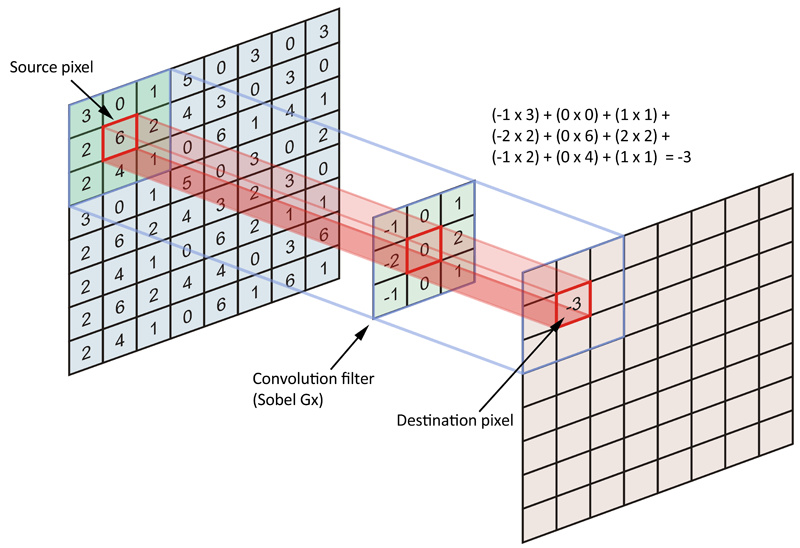
\includegraphics[width=0.7\textwidth]{Figures/convolucion.jpeg}
	\caption{Operacion de convolución \\ Fuente:  \href{http://openresearch.ai/t/network-in-network/39}{\textit{www.openresearch.ai}}}
	\label{convolucion}
\end{figure} 

\textbf{Componentes de la capa de convolución}
Las capas convolucionales poseen paramétros e hiperparametros. La gradiente de descenso se usa principalmente para entrenar los parametros de modo que las clases sean consistentes con las etiquetas en el conjunto de entrenamiento. Entre estos parámetros tenemos:
\textbf{Filtros}

Los filtros son una función que posee ancho(width) y alto (height) más pequeños que la entrada. Los filtros son aplicados a través de  del ancho y alto de la entrada. También pueden ser aplicados a la profundidad.
\subsubsection{Classification layers}

\subsection{Arquitecturas conocidas}
\section{Métodos de optimización}
Los métodos de optimización dentro del campo de deep learning son muy importantes debido a que esistentes gran cantidad de parámetros es 

\subsection{Gradiente de descenso}
La gradiente de descenso es un algoritmo común para optimizar redes neuronales. La gradiente de descenso es una forma de minimizar la función de costo $J(\theta)$ para metrizada por los parámetros $\theta \in\Re^{d}$ actualizando los parámetros en la dirección opuesta a la gradiente de la función objetivo en este caso a nuestra función de costo $\nabla_{\theta} J(\theta)$
Dentro de la gradiente de descenso podemos diferenciar 3 variantes de acuerdo al la cantidad de datos que se usan para calcular la gradiente de la función objetivo entre estas variantes tenemos a:\\
\subsubsection{Batch gradient descent}
Esta variante calcula la gradiente de descenso de la función de costo con respecto a un parámetro $\theta$, para todo el conjunto de datos. En la ecuación 4.1 podemos observar la actualización que se dará para cada ejecución. $\eta$ representa la taza o tamaño de los pasos para encontrar el mínimo local.
\begin{equation}
\label{bgds}
\begin{aligned}
\theta &= \theta - \eta \nabla_{\theta} J(\theta)
\end{aligned}
\end{equation}
La ecuación 4.1 asegura la convergencia para mínimo global en una supercifie convexa y mínimo local para una supercifie no convexa. Entre las dificultades de este método tenemos que puede llegar a ser lento y que esta limitado por la cantidad de datos ya que esta puede superar a la memoria del computador.	
\subsubsection{Stochastic gradient descent}
A diferencia del método anterior las actualización se realizan para cada ejemplo de entrenamiento de $(x^{i},y^{i})$ de esta manera se evitan problemas como la generación de redundancia debido a que se realiza una actualización por ejemplo de entrenamiento.
\begin{equation}
\label{sgds}
\begin{aligned}
\theta &= \theta - \eta \nabla_{\theta} J(\theta,x^{i},y^{i})
\end{aligned}
\end{equation}
En la figura 4.2 vemos que la función de costo en SGD fluctúa demasiado esto podría representar un problema pero al contrario de la figura representa que el método SGD es capaz de saltar de un mínimo local con lo cual puede encontrar mínimos locales potencialmente mejores.

\begin{figure}[H]
	\centering
	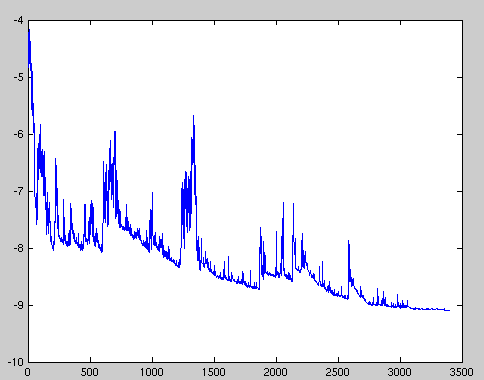
\includegraphics[width=0.5\textwidth]{Figures/sgd.png}
	\caption{Función costo en SGD \\ Fuente:  \href{https://www.doc.ic.ac.uk/~js4416/163/website/neural-networks/optimisers.html}{\textit{www.doc.ic.ac.uk}}}
	\label{funcion costo}
\end{figure} 

\subsubsection{Mini-batch gradient descent}
Este método pude verse como una mezcla de los 2 métodos anteriores, en lugar de aplicarlo para un conjunto entero de datos, los datos se particionan en pequeños conjuntos o mini batches.
Este método nos permite reducir la varianza de las actualizaciones de los parámetros lo cual nos permite una convergencia más estable. El tamaño de los mini-batches oscilan entre 50-250 y varían de acuerdo a su aplicación.

\begin{equation}
\label{mbgds}
\begin{aligned}
\theta &= \theta - \eta \nabla_{\theta} J(\theta,x^{i:i+n},y^{i:i+n})
\end{aligned}
\end{equation}



\subsection{Optimizadores}
En la siguiente sección analizaremos algunos optimizadores que acelerarán el proceso de gradiente de descenso.
\subsubsection{Momentum}
Las SGD tienen problemas para desplazarse en áreas con donde la superficie se curva más en una dimensión que en otra, estos lugares son los alrededores de los óptimos locales. En este escenario la SGD oscilará en la curvatura y descenderá lentamente hacia el óptimo como se muestra en la figura 4.3.
\begin{figure}[H]
	\centering
	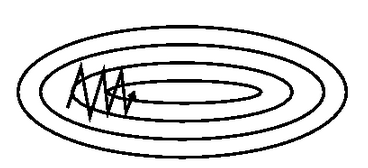
\includegraphics[width=0.5\textwidth]{Figures/momentum1.png}
	\caption{Actualización sin momentum \\ Fuente:  \href{https://www.doc.ic.ac.uk/~js4416/163/website/neural-networks/optimisers.html}{\textit{www.doc.ic.ac.uk}}}
	\label{momentum1}
\end{figure}
El momentum es un método que ayuda a la SGD a acelerar en la dirección correcta, mientras evitas las oscilaciones. El momentum lográ esto añadiendo una fracción $\gamma$ del vector de actualización pasado al vector presente tal como se muestra en las ecuaciones 4.4. Un valor comunmente elegido de $\gamma =0.9 $, en las actualización el valor del momentum aumenta para dimensiones cuyos gradientes apuntan en la misma dirección y disminuye para dimensional en la que la gradiente cambia de dirección. Esto nos asegura que tendremos una convergencia más rápida con una oscilación reducida.En la figura 4.4 se observa gráficamente la aceleración de la convergencia en la SGD.

\begin{equation}
\label{mbgds}
\begin{aligned}
\nu_{t}&=\gamma \nu_{t-1} +  \eta \nabla_{\theta} J(\theta)\\
\theta &= \theta -\nu_{t}
\end{aligned}
\end{equation}

\begin{figure}[H]
	\centering
	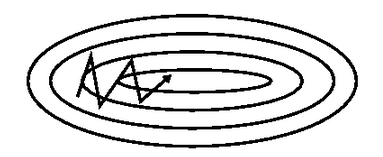
\includegraphics[width=0.5\textwidth]{Figures/momentum2.png}
	\caption{Actualización con momentum \\ Fuente:  \href{https://www.doc.ic.ac.uk/~js4416/163/website/neural-networks/optimisers.html}{\textit{www.doc.ic.ac.uk}}}
	\label{momentum2 }
\end{figure}

\subsubsection{Nesterov accelerated gradient}
Este método en el que nuestro descenso sea más controlado ya que reduce la velocidad antes de volver a subir una pendiente. En momentum usamos el término $\gamma \nu_{t-1}$ para mover los parámetros de $\theta$. Al calcular el valor de $\theta - \gamma \nu_{t-1}$ nos da una aproximación de donde se encontrá la siguiente posición de los parámetros. De esta forma no calculamos la gradiente en el parámetro $\theta$ actual sino que se calcula en una posición futura aproximada.




\begin{equation}
\label{mbgds}
\begin{aligned}
\nu_{t}&=\gamma \nu_{t-1} + \eta \nabla_{\theta} J(\theta- \gamma \nu_{t-1})\\
\theta &= \theta -\nu_{t}
\end{aligned}
\end{equation}

En la figura 4.5 observamos el proceso. Primero el momentum calcula  la gradiente actual(vector azul pequeño)  y luego da un gran salto en la dirección de la gradiente actualizada acumulada (gran vector azul), el NAG primero realiza un gran salto en dirección del gradiente acumulado previo(vector marron) luego realiza un correción(vector rojo), esto nos da como resultado la actualización completa de NAG(vector verde). Esta actualización anticipada es muy importante debido a que nos impide ir demasiado rápido y mejora la capacidad de respuesta lo cual aumenta el rendimiento de las CNN.
\begin{figure}[H]
	\centering
	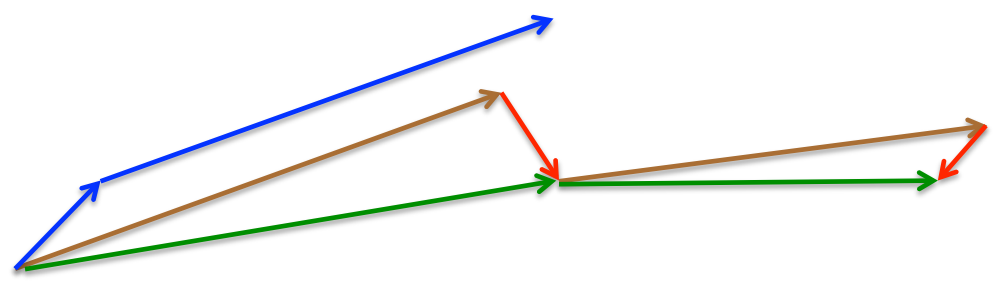
\includegraphics[width=0.5\textwidth]{Figures/nesterov.png}
	\caption{Convergencia Nesterov\\ Fuente:  \href{https://www.doc.ic.ac.uk/~js4416/163/website/neural-networks/optimisers.html}{\textit{www.doc.ic.ac.uk}}}
	\label{nesterov }
\end{figure}
\subsubsection{Adagrad}
Es una algoritmo optimización basada en la gradiente de descenso, el algoritmo adapta la tasa de aprendizaje  realizando actualizaciones más pequeñas para parámetros con carácteristicas que se repiten con más frencuencia y una tasa alta  para parámetros con carácteriscticas pocas frencuentes. Adagrad mejora en gran manera a la SGD, este método es usado para entrenar redes neuronales a gran escala. 

En métodos anteriores se usaba la actualización de todos los parámetros $\theta$ al mismo tiempo esto debido a que se usaba la misma tasa de aprendizaje $\eta $. Adagrad usa una tasa de aprendizaje diferente para cada parámetro $\theta_{i}$ en cada paso de tiempo $t$.
En la ecuación 4.6 
\begin{equation}
\label{adagrad1}
\begin{aligned}
g_{t,i}&=\nabla_{\theta} J(\theta_{t,i})\\
\theta_{t+1,i} &= \theta_{t,i} -\eta \cdot g_{t,i}
\end{aligned}
\end{equation}
El termino $\cdot g_{t,i}$ representa el valor de la gradiente en el paso de tiempo $t$, el cual es la derivada de la función objetivo con respecto al termino $\theta_{i}$.

Adagrad modifica la idea de utilizar una tasa $eta$ fija, podemos observar el la ecuación 4.7 es una variante de la ecuación 4.6. En donde se modifica la tasa de aprendizaje en cada paso de tiempo $t$ para todos los parámetros $\theta_{i} $basadas en los valores de las gradientes pasadas que fueron calculas para $\theta_{i}$
\begin{equation}
\label{adagrad2}
\begin{aligned}
\theta_{t+1,i} &= \theta_{t,i} - \frac{\eta}{\sqrt{G_{t,ii}+\epsilon}} \cdot g_{t,i}
\end{aligned}
\end{equation}

\begin{itemize}
	\item $G_{t,ii}$: representa la suma de los cuadrados de las gradientes pasadas con respecto a $\theta_{i}$
	\item $\epsilon $ es un término pequeño para evitar la división por 0. $\epsilon$ encuentra en el orden de $10^{-8}$.
\end{itemize}
Como $G_{t} \in \Re^{dxd} $contiene la suma de los cuadrados de las gradientes pasados con respecto a todos los parámetros de $\theta$ a lo largo de su diagonal. A lo largo  de su diagonal por lo cual se puede realizar ahora el producto matriz- vector.
\begin{equation}
\label{adagrad3}
\begin{aligned}
\theta_{t+1,i} &= \theta_{t,i} - \frac{\eta}{\sqrt{G_{t}+\epsilon}} \odot g_{t,i}
\end{aligned}
\end{equation}
El principal beneficio de adagrad nos evita el hecho de trabajar con una taza fija por otro lado su principal desventaja se basa en el la suma de los gradientes al cuadrado aumentará en cada iteración lo cual provocará que su taza sea cada vez más pequeña.


\subsubsection{RMSprop}
Es un método de aprendizaje por adaptación de la taza que fue propuesto por Geoff Hinton
Este modelo se desarrollo con el objetivo resolver el problema de disminuir radicalmente la tasa de aprendizaje en Adagrad. RMSprop divide la taza de aprendizaje mediante el decaimiento del promedio de la suma de las gradientes cuadradas.
\begin{equation}
\label{RMS}
\begin{aligned}
E[g^2]_{t} &= 0.9 E[g^2]_{t-1} + 0.1 g^{2}_{t}\\
\theta_{t+1} &= \theta_{t} - \frac{\eta}{\sqrt{E[g^2]_{t} +\epsilon }} g_{t}
\end{aligned}
\end{equation}

\subsubsection{Adam	}
Adaptative moment estimation  o Adam que calcula la taza de aprendizaje adaptativo para cada parámetro. Este método mantiene un decaimiento exponencial del promedio de las gradientes pasadas. El método adam prefiere los mínimos en las superficies de error. En la figura 4.9 mostramos el calculo de promedio de decaimiento de las gradientes pasadas $m_{t}$ y el cuadrado de las gradientes pasadas $v_{t}$
\begin{equation}
\label{adam1}
\begin{aligned}
m_{t} &= \beta_{1} m_{t-1} +(1-\beta_{1})g_{t} \\
v_{t} &= \beta_{2} v_{t-1} +(1-\beta_{2})g_{t}^2
\end{aligned}
\end{equation}

\begin{itemize}
	\item $m_{t}:$ Primer momento (media)
	\item $v_{t}:$ Segundo momento de la gradiente.
\end{itemize}

\begin{equation}
\label{adam2}
\begin{aligned}
\hat{m_{t}}&= \frac{m_{t}}{1-\beta_{1}^{t}} \\
\hat{v_{t}} &= \frac{v_{t}}{1-\beta_{2}^{t}}
\end{aligned}
\end{equation}
La ecuación 4.12 muestra la regla de actualización en Adam.
\begin{equation}
\label{adam3}
\begin{aligned}
\theta_{t+1}&= \theta_{t+1} - \frac{\eta}{\sqrt{\hat{v_{t}}}+\epsilon} \hat{m_{t}}	
\end{aligned}
\end{equation}

\subsubsection{AdaMax}
\subsubsection{Nadam}